%%%%%%%%%%%%%%%%%%%%%%%%%
\section{Experiments and Results}

\subsection{Experimental Setup}

\noindent\textbf{Datasets.} We consider the problem of finding social influencers in two domains: fashion and information technology (InfoTech). For both domains, we publish question-answering tasks in Figure Eight\footnote{\url{https://www.figure-eight.com}} and collect crowd workers' answers. Important statistics of these datasets are presented in Table~\ref{tab:datasets}. For both datasets, we randomly select 20\% of the candidate influencers and ask domain experts to label them. Our initial analysis reveals that the XX\% and XX\% of crowd answers are true influencers. Considering the relatively large number of crowd answers collected in a short period of time ($<$10 hours for both Fashion and InfoTech), this result validates our assumption that crowdsourced open-ended question-answering provides an efficient way for finding social influncers. Moreover, the sparsity of the answer matrix (Table~\ref{tab:datasets}) and the high percentage of incorrect answers motivates the necessity of open-ended answer aggregation that takes into account worker reliability.

\begin{table}[!ht]
%\small
\centering \caption{Descriptive statistics of the
datasets.}\label{tab:datasets}
%\vspace{-0.05in}
\addtolength{\tabcolsep}{-1mm}
\begin{tabular}{lcccc}
\toprule
    Datasets &\#Cand. Infl. &\#Workers &\#Answers &Sparsity   \\\midrule
    Fashion & & & & \\
    InfoTech & & & & \\
\bottomrule
\end{tabular}
% \vspace{-0.1in}
\end{table}

\smallskip
\noindent\textbf{Comparison Methods.} Due to the lack of existing open-ended answer aggregation methods, we compare with the following state-of-the-art closed-pool answer aggregation methods: 1) MV \cite{sheng2008get}, majority voting; 2) ZenCrowd \cite{demartini2012zencrowd}, EM method that estimates worker reliability as a model parameter; 3) Dawid-Skene \cite{dawid1979maximum}, EM method that learns worker reliability as a confusion matrix; 4) GLAD \cite{whitehill2009whose}, EM method that simutaneously learn worker reliability and task difficulty. To apply these methods to our problem, we use negative sampling to simulate workers' answers of non-influencers; we empirically find the optimal sampling rates for each comparison method. 

For \sys, we compare the following variants. a) LR: simplified \sys with only a logistic regression model trained on the labeled subset of candidate influencers for influencer classification; 2) NN: simplified \sys with only a multi-layer perceptron; 3) \sys-EM: \sys that further leverages worker answer matrix however models worker reliability as a fixed paramter; 4) \sys, the Bayesian version that models worker reliability as a latent variable.

\smallskip
\noindent\textbf{Parameter Settings.} The parameters of our framework and those for model training are empirically set. We search for the best model architecture for NN, and the predictor $f$ in \sys-EM and \sys with 0, 1, and 2 hidden layers, and apply a grid search in \{64, 128, 256, 512, 1024\} for the dimension of the hidden layesr. In model training, we select learning rates from \{0.0001, 0.001, 0.01, 0.1, 1\} for the learning of $\mathbf{W}_I$ in all variants of our framework, as well as for the learning of $r_j$ in \sys-EM. To investigate the impact of negative sampling, we experiment with sampling rate ($s\_rate$) from \{0, 1, 5, 10, 20, 50, 100\} where $s\_rate=5$ indicates that for each worker, the negative samples is five times the size of the candidate influencers named by the worker. 

\smallskip
\noindent\textbf{Evaluation Protocals.} We split the labeled subset of candidate influencers into training, validation, and test sets. \sys is trained on the answer matrix and the training set, and evaluated on the test set. Validation set is used to search for the optimal parameter settings. To investigate the impact of the degree of supervision ($s\_deg$) on \sys performance, we split the labeled subset by $s\_deg\in \{50\%, 60\%, 70\%, 80\%, 90\%\}$, where $s\_deg = 60\%$ means that 60\% of the labeled subset is used for training, and the rest for validation and test with equal split.



\subsection{Results of \sys}
\label{sec:selfres}

\noindent\textbf{Results of \sys Variants.}
\begin{figure}[htb]
\begin{subfigure}[t]{0.47\columnwidth}
        \centering
    \pgfplotstableread[row sep=\\,col sep=&]{
       cases & LR & NN & EM & VEM \\
       Fashion     & 0.6027  & 0.7006  & 0.7194 &0.7472  \\
       IT    & 0.7567 & 0.7742  & 0.7829 &0.7932 \\
    }\mydata

    \begin{tikzpicture}[scale=0.5]
    \begin{axis}[
    ybar,
    bar width=.55cm,
    width=2\textwidth,
    height=1.5\textwidth,
    legend style={at={(0.67,1.2)},
       anchor=north,legend columns= 4, font = \LARGE},
    symbolic x coords={Fashion, IT},
    xtick=data,
    enlarge x limits=0.3,
    ymin=0.60,ymax=0.80,
    ylabel={Accuracy},
    yticklabel style = {font=\huge,xshift=0.5ex},
    xticklabel style = {font=\huge,yshift=0.5ex},
    ylabel style ={font = \huge},
    ymajorgrids=true
    ]
    \addplot[draw=gray,fill=gray!40!white, thick] table[x=cases,y=LR]{\mydata};
    \addplot[draw=blue,fill=blue!40!white] table[x=cases,y=NN]{\mydata};
    \addplot[draw=black,fill=black!50!white, thick] table[x=cases,y=EM]{\mydata};
    \addplot[draw=red,fill=red!40!white, thick] table[x=cases,y=VEM]{\mydata};
    \legend{LR, NN, EM, VEM}
    \end{axis}
    \end{tikzpicture}
    \vspace{-0.15in}
        \caption{Accuracy\label{fig:acc}} 
    \end{subfigure}% 
  \hfill \hskip -2.5ex %
    	\begin{subfigure}[t]{0.47\columnwidth}
        \centering
  \centering
    \pgfplotstableread[row sep=\\,col sep=&]{
       cases & LR & NN & EM & VEM \\
       Fashion     &0.2228  & 0.2154  & 0.2467 &0.4235  \\
       IT   &0.2228  & 0.2154  & 0.2467 &0.4235 \\
    }\mydata

    \begin{tikzpicture}[scale=0.5]
    \begin{axis}[
    ybar,
    bar width=.55cm,
    width=2\textwidth,
    height=1.5\textwidth,
    legend style={at={(0.67,1.2)},
       anchor=north,legend columns= 4, font = \LARGE},
    symbolic x coords={Fashion, IT},
    xtick=data,
    enlarge x limits=0.3,
    ymin=0.2,ymax=0.5,
    ylabel={AUPRC},
    yticklabel style = {font=\huge,xshift=0.5ex},
    xticklabel style = {font=\huge,yshift=0.5ex},
    ylabel style ={font = \huge},
    ymajorgrids=true
    ]
    \addplot[draw=gray,fill=gray!40!white, thick] table[x=cases,y=LR]{\mydata};
    \addplot[draw=blue,fill=blue!40!white] table[x=cases,y=NN]{\mydata};
    \addplot[draw=black,fill=black!50!white, thick] table[x=cases,y=EM]{\mydata};
    \addplot[draw=red,fill=red!40!white, thick] table[x=cases,y=VEM]{\mydata};
    \legend{LR, NN, EM, VEM}
    \end{axis}
    \end{tikzpicture}
    \vspace{-0.15in}
        \caption{AUPRC\label{fig:auprc}} 
    \end{subfigure}% 
   \caption{\sys performance} \label{fig:variants}
\end{figure}
\iar{IT values to be replaced!!}
\smallskip
\noindent\textbf{Benefits of Incorporating Confidence.}

\smallskip
\noindent\textbf{Impacts of Sampling Rate.}



\begin{figure}[htb]\centering
	\begin{subfigure}[t]{0.47\columnwidth}
        \centering
        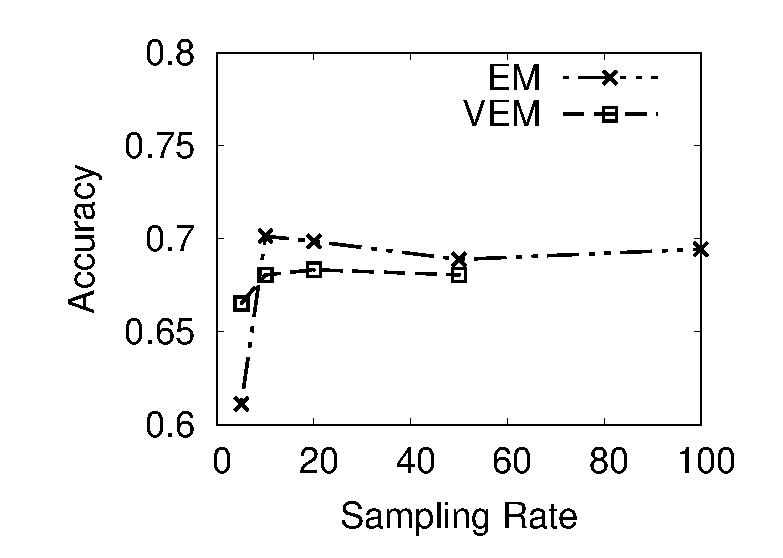
\includegraphics[width=\columnwidth]{figs/accuracy}
        \caption{Accuracy with varying sampling rate\label{fig:accuracy}} 
    \end{subfigure}% 
  \hfill \hskip -2.5ex %
    	\begin{subfigure}[t]{0.47\columnwidth}
        \centering
        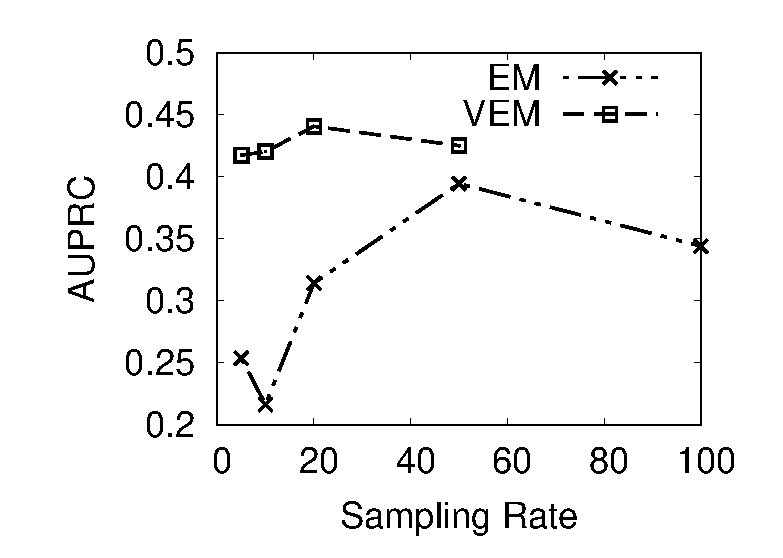
\includegraphics[width=\columnwidth]{figs/auprc}
        \caption{AUPRC with varying sampling rate\label{fig:auprc}} 
    \end{subfigure}% 
    \caption{Fashion Data}
    \vspace{-5mm}
  \label{fig:sys_perf} 
\end{figure}
\iar{some values are still running!}
\subsection{Comparative Results}
\label{sec:compres}


\smallskip
\noindent\textbf{Impacts of Supervision Degree.}

